\documentclass{standalone}
\usepackage[dvipsnames]{xcolor}
\usepackage{pgfplots}
\pgfplotsset{
  compat=1.18, 
  trig format=rad, 
  ticklabel style = {font=\tiny},
  axis equal image,
}

\begin{document}
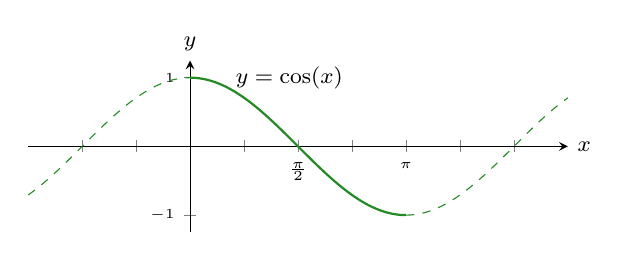
\begin{tikzpicture}
  \begin{axis}[
    xlabel={\footnotesize \(x\)},
    ylabel={\footnotesize \(y\)},
    xmin={-pi-pi/4+pi/2},
    xmax={pi+pi/4+pi/2},
    ymin={-1.25},
    ymax={1.25},
    axis x line={middle},
    axis y line={middle},
    xlabel style={at={(ticklabel* cs:1)}, anchor=west},
    ylabel style={at={(ticklabel* cs:1)}, anchor=south},
    ytick={-1,0,1},
    xtick={-pi+pi/2, -3*pi/4+pi/2, -pi/2+pi/2, -pi/4+pi/2, 0+pi/2, pi/4+pi/2, pi/2+pi/2, 3*pi/4+pi/2, pi+pi/2},
    % yticklabels={,,},
    xticklabels={,,,,\(\frac{\pi}{2}\),,\(\pi\)}
    ]

    % \addplot[thick, smooth, samples=1000, domain=-1:1] {asin(x)/180*pi};
    \addplot[ForestGreen, thick, smooth, samples=1000, domain={-pi/2+pi/2}:{pi/2+pi/2}] {cos(x)};
    \addplot[ForestGreen, dashed, smooth, samples=1000, domain={-pi-pi/4+pi/2}:{-pi/2+pi/2}] {cos(x)};
    \addplot[ForestGreen, dashed, smooth, samples=1000, domain={pi/2+pi/2}:{pi+pi/4+pi/2}] {cos(x)};
    \node[right] at ({0+pi/6}, 1) {\footnotesize \(y = \cos(x)\)};
  \end{axis}
\end{tikzpicture}
\end{document}
